% STALE AFTER THE 2026-09-16 CHANGE OF RUNNING EXAMPLE: names and tool set were updated to
% mini-swe-agent, but any claim about tests as an oracle still needs rewriting before reuse.
% Removed from Section 1 on 2026-09-16 at Rahul's request: AIMA S2.4.7's atomic, factored, and structured
% representations, mapped onto mini-swe-agent (result label, state record, patch and test failure).
% Intended for Part B's state-schema section, where factored state has a consequence (one reducer per
% field; mechanical validation over named fields). Not input by lecture_notes.tex.

\subsection{How the components of agent programs work}
\label{sec:agents-components}

The components of an agent program answer questions such as what the world is like now and what
action to do now, and the ways they can represent the environment lie on an axis of increasing
expressive power: atomic, factored, and structured \citep[\S2.4.7]{russell2020aima}. In an
atomic representation each state is indivisible, a black box whose only property is being the
same as or different from another. A factored representation splits each state into a fixed set
of variables or attributes, each with a value. A structured representation describes objects,
each with attributes of its own and relationships to other objects.

\begin{figure}[htbp]
  \centering
  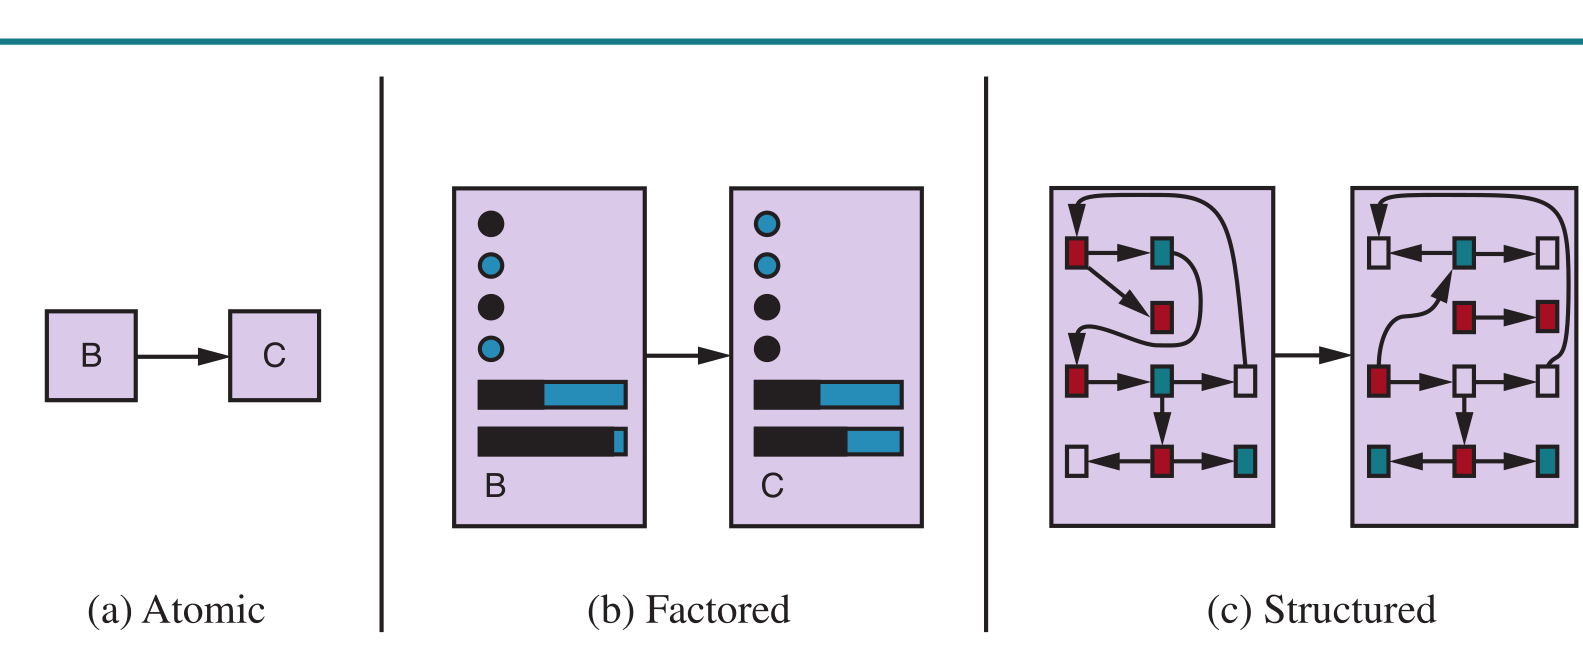
\includegraphics[width=0.75\linewidth]{figures/aima-fig2-16.png}
  \caption{Three ways to represent states and the transitions between them. Figure~2.16 of
  \citet{russell2020aima}, reproduced from the Global Edition (\copyright~Pearson Education
  Limited 2022).}
  \label{fig:agents-fig216}
\end{figure}

\msa{} uses all three, at different places.
\begin{itemize}
  \item \textbf{Atomic:} the run's outcome. Resolved or not resolved is a label with no
  internal structure, and two runs that end in the same label are indistinguishable at this
  level. The leaderboard number a benchmark reports is a count of such labels.
  \item \textbf{Factored:} the state record. The instance, the locations found, the excerpts
  read, the edits applied, the the Submit state's checks, the calls and tokens spent, and the investigation
  status are variables with values, and two states can share some values and differ in others.
  This is the state schema of every version in this block, and it is what makes one reducer per
  field (\cref{sec:reactive}) possible.
  \item \textbf{Structured:} the patch and the failure. A patch is a set of hunks, each over a
  file and a range of lines; a rejected submission names the check that failed, the file, and the line. Both are objects with relations to other objects, and
  a patch whose hunks touch no line that the failure names is one the validator of
  \cref{sec:validation} questions.
\end{itemize}
A more expressive representation captures everything a less expressive one can and is often
more concise, but reasoning and learning over it are more complex
\citep[\S2.4.7]{russell2020aima}. That is why we keep the state factored and let only the patch
and the test output be structured: the runtime can validate and route over named fields, and
the structure lives where the model has to defend it.

